% PREAMBLE ====
\documentclass[preprint,5p]{elsarticle} % TODO: What model?

% Use times font
\usepackage{mathptmx}
\usepackage{lmodern}
\usepackage{times}
\usepackage{soul} % For highlighting

% Math
\usepackage{amsmath}

% Tables
\usepackage{booktabs}
\usepackage{threeparttable}
% For line-breaking cells
\newcommand{\spc}[2][c]{%
  \begin{tabular}[#1]{@{}l@{}}#2\end{tabular}}
% Reduce table spacing
\setlength{\tabcolsep}{10pt}

% Figures
\usepackage{float}
% Reset numbering for supplementary figures
\usepackage{newfloat}
\DeclareFloatingEnvironment[name={Supplementary Figure}]{suppfigure}
\usepackage{caption}

% Graphics
\usepackage{graphicx}
\DeclareGraphicsExtensions{.pdf,.png}
\graphicspath{{../../figures/}}

% References
\usepackage{numcompress}
\biboptions{super}
\bibliographystyle{model3-num-names}

% DOCUMENT ====
\begin{document}
% FRONTMATTER ====
\begin{frontmatter}
\title{Parkinson's Disease cluster analysis}
% \author[c3]{Pablo Martinez-Martin}
% \ead{pmartinez@isciii.es}
% \author[bc]{Jesse Mu}
% \ead{muj@bc.edu}
% \author[cig]{Concha Bielza}
% \ead{mcbielza@fi.upm.es}
% \author[cig]{Pedro Larra\~naga}
% \ead{plarranaga@fi.upm.es}
% \address[c3]{Area of Applied Epidemiology, National Centre of Epidemiology and CIBERNED, Carlos III Institute of Health, Madrid, Spain}
% \address[bc]{Department of Computer Science, Boston College, Chestnut Hill, Massachusetts, USA}
% \address[cig]{Computational Intelligence Group, Polytechnic University of Madrid, Madrid, Spain}

\begin{abstract}
\emph{Background} \quad This is the background. \\
\emph{Methods} \quad  These are methods. \\
\emph{Findings} \quad These are findings. \\
\emph{Interpretation} \quad This is interpretation. \\
\emph{Funding} \quad This is funding.
\end{abstract}
\journal{The Lancet Neurology}
\end{frontmatter}

% BODY ====

\section{Introduction}

\section{Methods}

\subsection{Statistical analysis}

Out of the 951 patients in the study, we used listwise deletion to exclude 47 patients due to
missing measurements in the variables of interest, resulting in 904 remaining patients. All
symptoms were standardized before clustering, and unstandardized afterwards for
interpretation.
Analyses were conducted in R version 3.2.4 (www.r-project.org).

\subsubsection{Cluster analysis}

$k$-means was used for cluster analysis. We performed two analyses on the
patients in the dataset: the first ``domains clustering'' on the nine aggregate nonmotor symptom
domains and the four motor symptoms, and the second ``symptoms clustering'' on the 30 individual
nonmotor symptoms collected with the four motor symptoms. Complete-linkage
hierarchical agglomerative clustering on the 30 nonmotor symptoms was also performed to how the symptoms group
together.

\subsubsection{Determining $k$}

Various formal measures were used to determine the optimal number of clusters for the dataset. The
optimal $k$ according to the Gap Statistic and the 1-standard-error method suggested by
Tibshirani\cite{tibshirani01gap} was $k = 4$ (Supplementary Figure~\ref{fig:gap}). Other cluster validation
methods (within sum of squares error scree plot, minimum average silhouette width) suggested $k =
2, 3, 4$, where $k = 2, 3$ simply divided the data uninformatively into groups with varying levels
of overall PD severity. Thus $k = 4$ was selected to offer a good blend of model fit,
informativeness, and parsimony.

\subsubsection{Interpretation}

For the domains clustering, we displayed the distribution of each symptom for the four
clusters using boxplots, which allowed us to visualize the center and spread of each cluster. Since
the number of variables was larger for the symptoms clustering, we visualized results for the
second analysis with a heatmap. Finally, for the hierarchical clustering on the symptoms
themselves, we displayed results in a dendrogram and clustered the symptoms into four interpretable
clusters.

For each symptom in both clusterings, we used one-way ANOVA and $\chi^2$ tests to respectively
check the equality of symptom means and proportions across the clusters found, using Bonferroni
correction for multiple testing with corrected $p < 0.05$ considered significant. Differences among
pairwise clusters were tested post-hoc using Tukey's range test for continuous means, or pairwise
$\chi^2$ tests with Bonferroni correction for proportions.

To compare the clusterings, we visualized cluster alignment with stacked barplots, and computed the adjusted rand index\cite{hubert1985} (ARI) and
Rosenberg's $v$-measure\cite{rosenberg07vmeasure} to evaluate similarity between the two
clusterings. Both measures range from 0 (no similarity) to 1 (identical), and respectively take a
contingency table and information-theoretic approach to measuring clustering similarity.

Lastly, to explore the relationship between symptom severity and disease duration, we computed the
correlation coefficient for each symptom with PD duration and fitted smoothed loess curves to the
data both globally and for each cluster found in the previous analyses.

\section{Results}

\subsection{Domains clustering}

Results from the clustering on the nine nonmotor domains and the four motor symptoms, as well as
additional variables not used in the analysis, are reported in Table~\ref{tab:nmd}, with boxplots
in Figure~\ref{fig:box}.
Cluster means for all variables were found to be statistically different, except for PD onset ($p <
0.05 / 18 \approx 0.003$ after correcting for the comparisons of the 18 variables). Specific
pairwise differences are noted in the table.

Cluster 1 ($n = 406$) patients were mildly affected in all domains. This cluster was characterized
by relatively lower disease durations and ages.

Cluster 2 ($n = 189$) patients were severely affected in nonmotor domains but mildly affected in
motor domains. This cluster had an incidence of motor symptoms relatively similar to the Cluster 1
(mild) subtype especially in tremor, but generally expressed significantly higher scores for
nonmotor symptoms than Clusters 1 and 3, especially in the sleep/fatigue, mood/apathy and
miscellaneous domains. This group also had a statistically higher percentage of females than
Cluster 3.
% But also high variability

Cluster 3 ($n = 221$) patients were severely affected in motor domains but mildly affected in
nonmotor domains. Mean motor scores were greater than the means of clusters 1 and 2, but less than
4, with the exception of tremor, which was especially high.

Cluster 4 ($n = 88$) patients were severely affected in all domains, having the greatest symptom
mean out of all four clusters with the exception of tremor. Consequently, patients in Cluster 4 had
the longest average PD duration and oldest ages, but did not have a significantly different age of
PD onset.

\begin{table*}[t]
  \centering
  \caption{Domains clustering summary. Unless otherwise specified, statistics are
  reported as mean (sd).}
  \label{tab:nmd}
  \begin{threeparttable}
    \small
    \begin{tabular}{lrllll}
    \toprule
    	 Cluster 	 1 	 2 	 3 	 4 \\
    	 $n$ 	 406 (45\%) 	 189 (21\%) 	 221 (24\%) 	 88 (10\%) \\
    \midrule
    Nonmotor domains 	 Cardiovascular 	 0.7 (1.6)\tnote{24} 	 2.3 (2.9)\tnote{134} 	 1.1 (2.0)\tnote{24} 	
    7.0 (6.0)\tnote{123} \\
    a	 Sleep/fatigue 	 4.3 (4.8)\tnote{234} 	 14.9 (8.2)\tnote{134} 	 6.9 (6.3)\tnote{124} 21.0 (10.0)\tnote{123} \\
  	 a  Mood/apathy 	 3.1 (4.5)\tnote{234} 	 16.1 (14.0)\tnote{134} 	 6.6 (8.1)\tnote{124} 	 23.4 (14.3)\tnote{123} \\
    	 Perception/hallucination 	 0.5 (1.7)\tnote{24} 	 1.9 (3.5)\tnote{134} 	 0.8 (2.0)\tnote{24} 	 8.6 (6.9)\tnote{123} \\
    	 Attention/memory 	 2.8 (4.2)\tnote{24} 	 8.9 (8.1)\tnote{134} 	 3.2 (4.4)\tnote{24} 	15.6 (11.1)\tnote{123} \\
    	 Gastrointestinal 	 2.8 (3.9)\tnote{234} 	 8.8 (7.1)\tnote{134} 	 4.1 (4.7)\tnote{124} 	 14.6 (9.6)\tnote{123} \\
    	 Urinary 	 4.5 (5.9)\tnote{234} 	 12.4 (9.7)\tnote{134} 	 6.1 (6.4)\tnote{124} 	20.3 (9.9)\tnote{123} \\
    	 Sexual function 	 1.5 (3.1)\tnote{24} 	 6.4 (7.4)\tnote{134} 	 2.5 (4.1)\tnote{24} 	9.0 (9.7)\tnote{123} \\
    	 Miscellaneous 	 3.9 (4.7)\tnote{24} 	 13.2 (8.6)\tnote{13} 	 5.2 (5.8)\tnote{24} 	14.0 (9.5)\tnote{13} \\
    \midrule
    Motor symptoms 	 Tremor 	 1.9 (1.8)\tnote{34} 	 1.6 (1.9)\tnote{34} 	 4.3 (2.8)\tnote{124} 	 3.5 (3.8)\tnote{123} \\
    	 Bradykinesia 	 1.5 (0.9)\tnote{234} 	 2.1 (1.1)\tnote{134} 	 3.6 (0.9)\tnote{124} 	4.0 (1.5)\tnote{123} \\
    	 Rigidity 	 1.5 (0.9)\tnote{234} 	 1.8 (1.1)\tnote{134} 	 3.3 (0.9)\tnote{124} 	3.8 (1.4)\tnote{123} \\
    	 Axial 	 1.8 (1.6)\tnote{234} 	 3.3 (2.1)\tnote{134} 	 4.3 (2.4)\tnote{124} 	7.4 (2.9)\tnote{123} \\
    \midrule
    Variables not 	 Sex (\% male) 	 63 	 53\tnote{3} 	 71\tnote{2} 	 58 \\
    used in analysis 	 CISI total 	 5.7 (3.2)\tnote{234} 	 9.2 (3.9)\tnote{14} 	 9.7 (3.5)\tnote{14} 	 14.8 (5.1)\tnote{123} \\
    	 Age (34--89) 	 62.7 (9.7)\tnote{34} 	 64 (9.0)\tnote{4} 	 65 (10.2)\tnote{14} 	 70.5 (8.9)\tnote{123} \\
    	 PD onset 	 56 (10.6) 	 55.2 (10.1) 	 56.9 (11.1) 	 58.2 (11.4) \\
    	 PD duration 	 6.7 (4.8)\tnote{234} 	 8.7 (5.7)\tnote{14} 	 8 (5.5)\tnote{14} 	12.3 (8.1)\tnote{123} \\
    \bottomrule
  \end{tabular}
  \begin{tablenotes}
    \small
    \item[1] Significant difference with cluster 1 (corrected $p < 0.05$)
    \item[2] Significant difference with cluster 2 (corrected $p < 0.05$)
    \item[3] Significant difference with cluster 3 (corrected $p < 0.05$)
    \item[4] Significant difference with cluster 4 (corrected $p < 0.05$)
  \end{tablenotes}
  \end{threeparttable}
\end{table*}

\begin{figure*}[b]
  \centering
  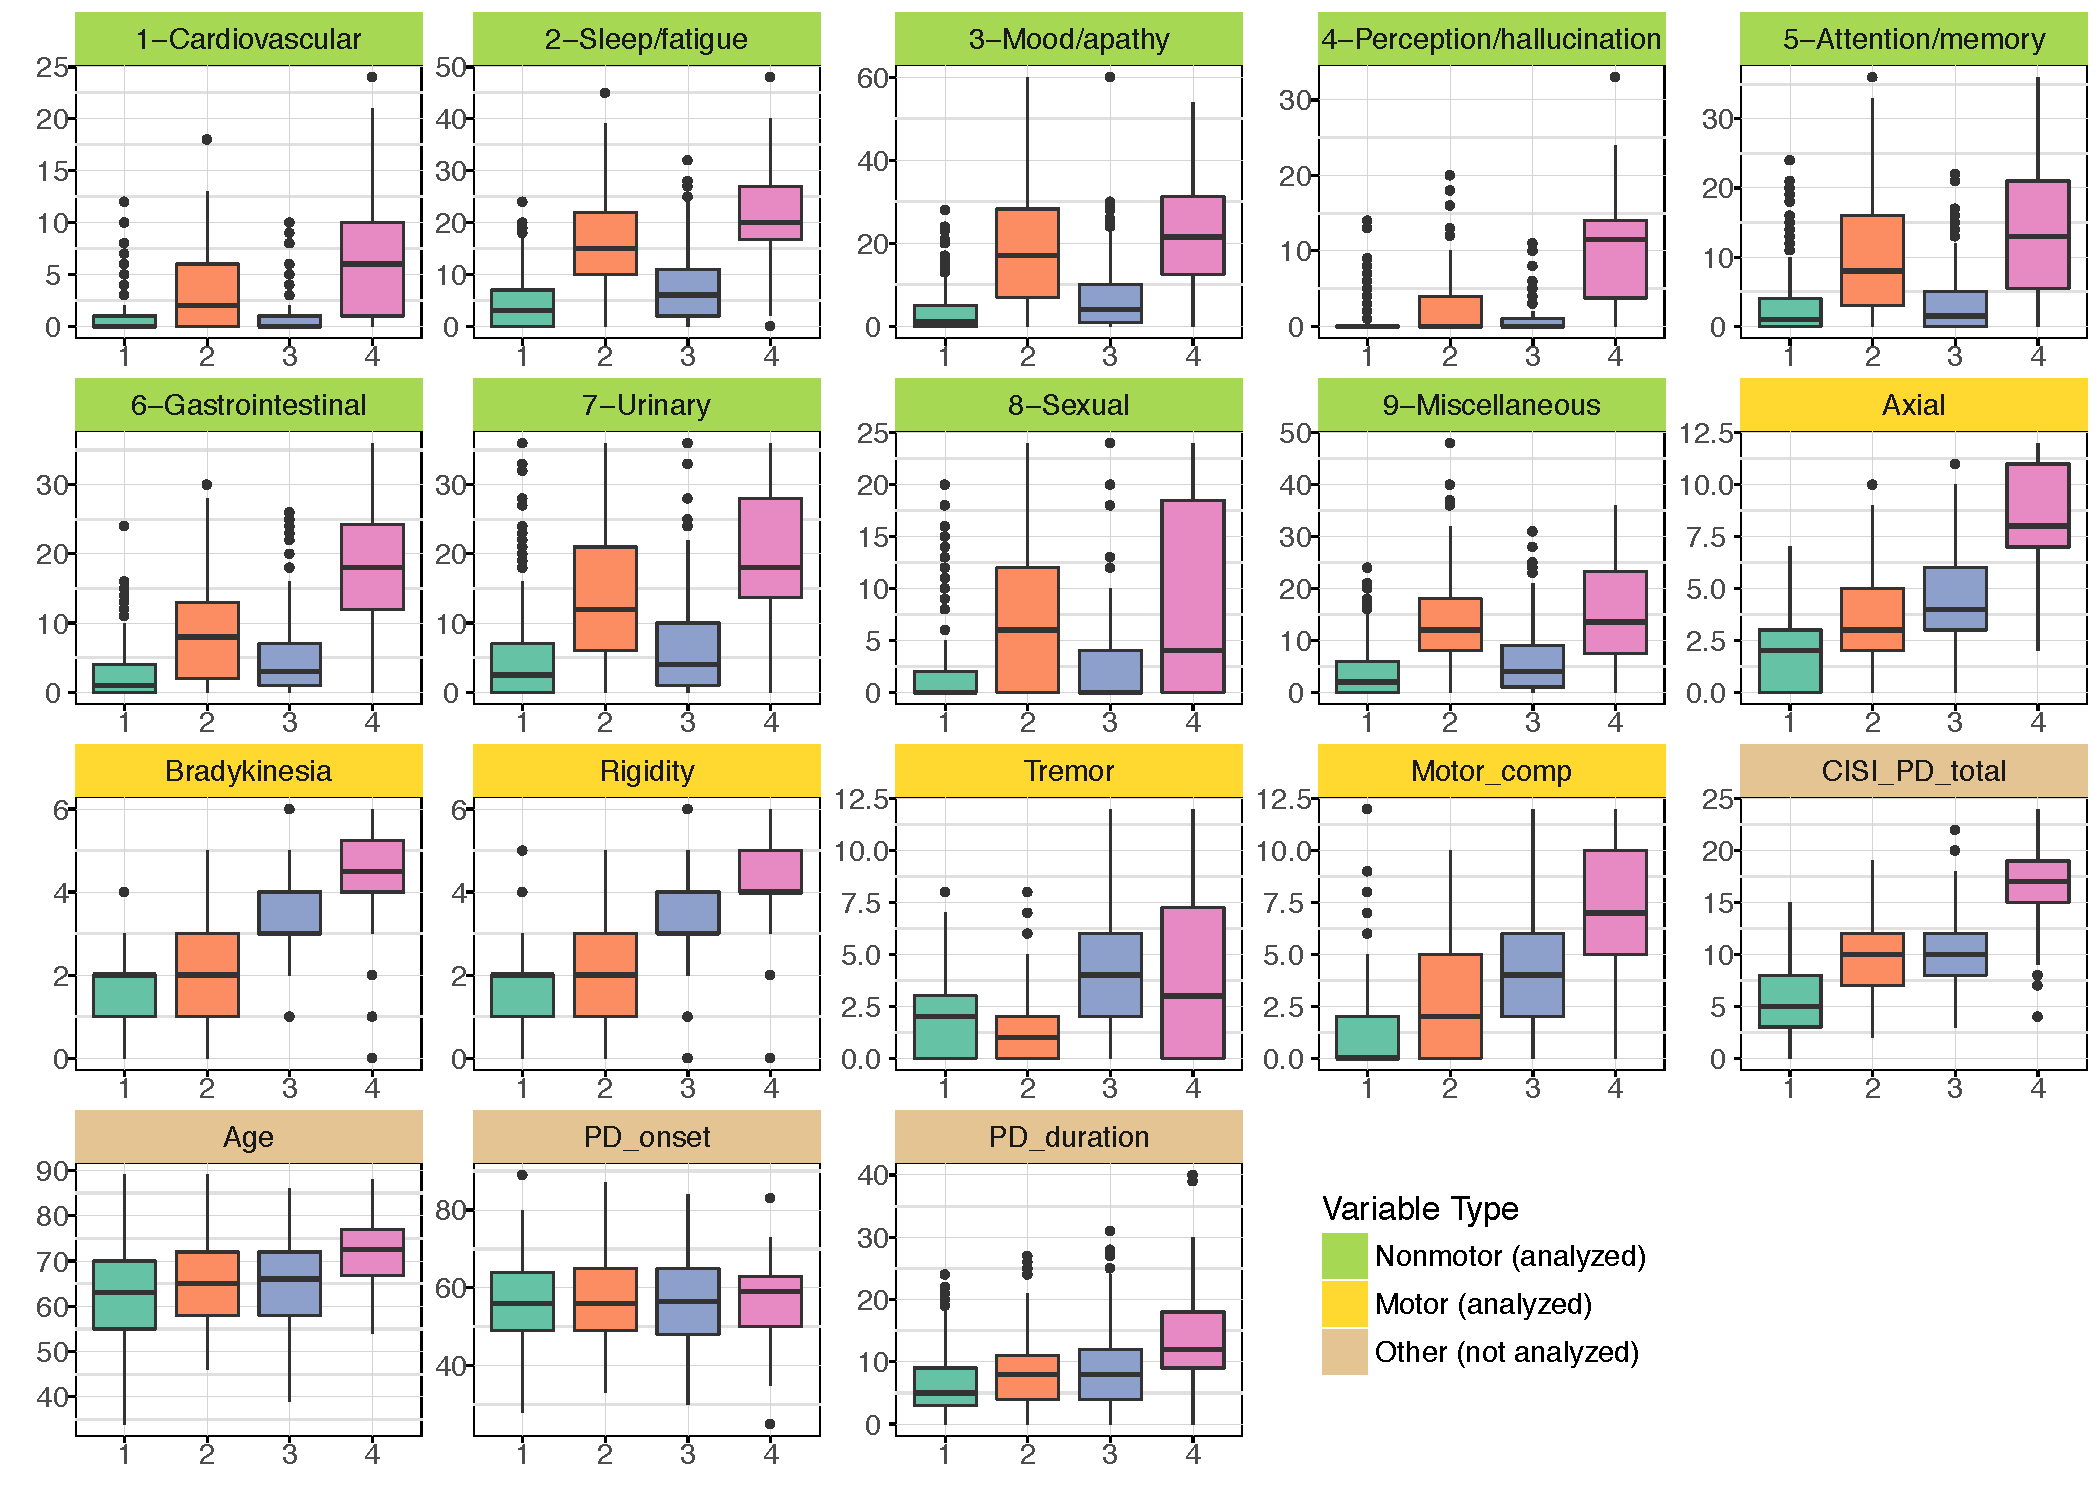
\includegraphics[width=\linewidth]{kmeans-summaries-4-pub.pdf}
  \vspace{-7.5em}
  \captionsetup{justification=raggedleft,
    singlelinecheck=false
  }
  \caption{Boxplots for domains clustering.}
  \label{fig:box}
\end{figure*}

\subsection{Symptoms clustering}

$k$-means clustering performed on the 30 individual nonmotor symptoms found similar patterns to the
first clustering {(Table~\ref{tab:nms30}, heatmap in Figure~\ref{fig:nms30-hm}). Means of all
symptoms were found to differ across clusters except for PD onset and tremor.

Clusters 1 ($n = 509$) and 4 ($n = 49$), the mild and severe subtypes of the previous clustering,
retained their characteristics here, while clusters 2 ($n = 97$) and 3 ($n = 249$) were
characterized differently.
Cluster 2 was a mood/apathy-dominant cluster, with a relatively higher proportion of female patients and
additionally a more severe incidence of insomnia. Cluster 3 was not characterized by any especially high
symptoms and was thus classified as a group of patients with average severity.
% Once again, CISI TOTAL...

\subsection{Comparison between clusterings}

 The two clusterings were somewhat similar ($\text{ARI} = 0.46$; $\text{$v$-measure} = 0.43$). To
 help compare the alignment of the two clusterings, we denoted the four clusters in the domains
 clustering as $D_1, D_2, D_3, D_4$, and the clusters in the symptoms clustering as $S_1, S_2, S_3,
 S_4$.
Alignment of the clusters is visualized in Figure~\ref{fig:align}. While clusters $D_1/S_1$ and
$D_4/S_4$
aligned well with each other, main differences in the clusterings occurred in the mixing of
clusters 2 and 3; for example, $D_3$ (motor-dominant) was somewhat
evenly split among $S_1$ (mild) and $S_3$ (average).}

\begin{figure}[H]
  \centering
  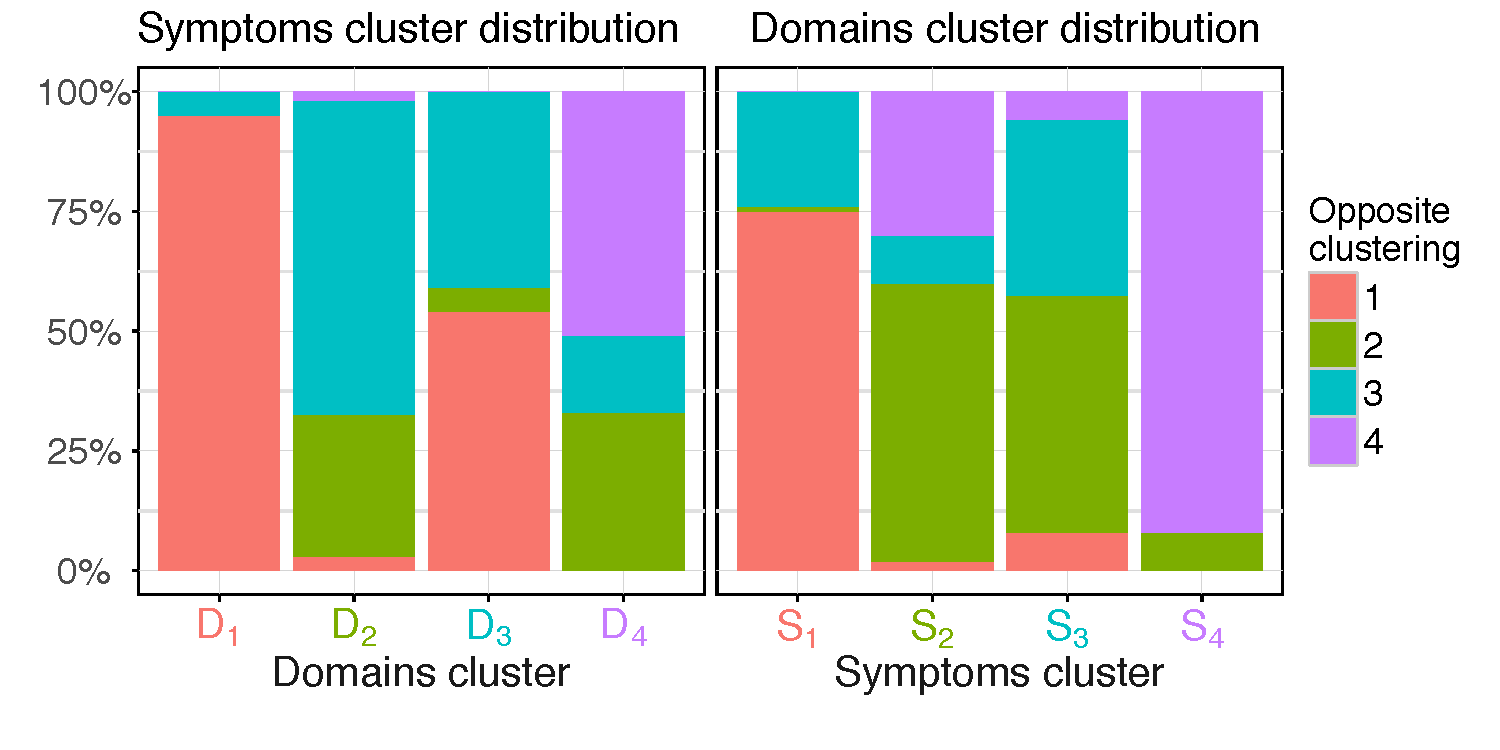
\includegraphics[width=\linewidth]{cluster-alignment.pdf}
  \caption{Stacked barplots indicating the distribution of opposite cluster membership for the patients of
  a given cluster. For example, the bar furthest left indicates that close to 100\% of patients in
domains cluster 1 are in symptoms cluster 1, with the rest in symptoms cluster 3.}
  \label{fig:align}
\end{figure}

% Perhaps this table belongs in appendix?
\begin{table*}[t]
  \centering
  \caption{Summaries of clustering on individual nonmotor domains. Unless otherwise specified,
  statistics are reported as mean (sd).}
  \label{tab:nms30}
  \begin{threeparttable}
  \small
\begin{tabular}{lrllll}
  \toprule
    & Cluster & 1 & 2 & 3 & 4 \\
    & $n$ & 509 (56.3\%) & 97 (10.7\%) & 249 (27.5\%) & 49 (5.4\%) \\
  \midrule
  1.\ Cardiovascular &
  Lightheadedness & 0.6 (1.3)\tnote{234} & 2.4 (3.0)\tnote{14} & 2.1 (2.9)\tnote{14} & 5.2
  (4.2)\tnote{123} \\
  &Fainting & 0.1 (0.7)\tnote{24} & 0.5 (1.4)\tnote{134} & 0.2 (0.6)\tnote{24} & 2.4
  (3.5)\tnote{123} \\
  \midrule
  2.\ Sleep/fatigue &
  Drowsiness & 1.0 (1.9)\tnote{234} & 2.8 (3.3)\tnote{14} & 2.5 (3.0)\tnote{14} & 7.0
  (3.8)\tnote{123} \\
  &Fatigue & 1.3 (2.0)\tnote{234} & 6.3 (4.2)\tnote{13} & 4.8 (3.9)\tnote{124} & 7.3 (3.5)\tnote{13} \\
  &Insomnia & 1.2 (2.6)\tnote{234} & 5.5 (4.8)\tnote{13} & 3.2 (3.8)\tnote{12} & 4.2
  (3.9)\tnote{1} \\
  &RLS & 0.7 (1.6)\tnote{234} & 2.3 (3.5)\tnote{14} & 1.9 (3.2)\tnote{14} & 3.9
  (3.9)\tnote{123} \\
  \midrule
  3.\ Mood/apathy &
  Loss\_interest & 0.4 (1.1)\tnote{234} & 6.1 (3.8)\tnote{134} & 1.0 (1.8)\tnote{124} & 4.6 (3.7)\tnote{123} \\
  &Loss\_activities & 0.7 (1.6)\tnote{234} & 7.1 (4.1)\tnote{134} & 1.7 (2.4)\tnote{124} &
  5.4 (4.0)\tnote{123} \\
  &Anxiety & 0.9 (1.8)\tnote{234} & 6.6 (4.3)\tnote{134} & 2.0 (2.8)\tnote{124} & 4.6 (3.9)\tnote{123} \\
  &Depression & 0.8 (1.6)\tnote{234} & 7.8 (3.7)\tnote{134} & 2.3 (3.0)\tnote{124} & 4.3 (3.7)\tnote{123} \\
  &Flat\_affect & 0.4 (1.1)\tnote{234} & 4.9 (4.3)\tnote{134} & 0.9 (1.9)\tnote{124} & 2.7 (3.0)\tnote{123} \\
  &Loss\_pleasure & 0.4 (1.2)\tnote{234} & 6.8 (4.1)\tnote{134} & 1.1 (2.1)\tnote{124} & 3.4 (3.3)\tnote{123} \\
  \midrule
  % This one is spread across multiple cells
  4.\ Perception/ & Hallucination & 0.2 (1.0)\tnote{234} & 0.8 (1.9)\tnote{14} & 0.6 (1.6)\tnote{14} & 4.6 (3.6)\tnote{123} \\
  hallucination &Delusion & 0.1 (0.7)\tnote{24} & 1.5 (3.1)\tnote{124} & 0.2 (1.0)\tnote{24} &
  3.1 (3.8)\tnote{123} \\
  &Diplopia & 0.2 (0.7)\tnote{234} & 1.0 (2.5)\tnote{14} & 0.6 (1.4)\tnote{14} & 4.4
  (4.3)\tnote{123} \\
  \midrule
  5.\ Attention/ & Loss\_concentration & 0.9 (1.8)\tnote{234} & 4.0 (3.6)\tnote{134} & 2.5 (3.1)\tnote{124} & 6.6 (3.9)\tnote{123} \\
  memory &Forget\_explicit & 0.9 (1.6)\tnote{234} & 3.8 (3.9)\tnote{134} & 2.2 (2.9)\tnote{124} & 6.7 (3.6)\tnote{123} \\
  &Forget\_implicit & 0.7 (1.6)\tnote{234} & 3.1 (3.7)\tnote{134} & 1.8 (2.6)\tnote{124} & 6.7 (4.0)\tnote{123} \\
  \midrule
  6.\ Gastrointestinal &
  Drooling & 0.7 (1.6)\tnote{234} & 3.0 (4.1)\tnote{14} & 3.0 (3.8)\tnote{14} & 6.1 (4.4)\tnote{123} \\
  &Swallowing & 0.4 (1.2)\tnote{234} & 1.2 (2.1)\tnote{14} & 1.7 (2.8)\tnote{14} & 4.5 (3.9)\tnote{123} \\
  &Constipation & 1.6 (2.9)\tnote{234} & 3.6 (4.3)\tnote{14} & 3.3 (4.1)\tnote{14} & 7.0 (5.1)\tnote{123} \\
  \midrule
  7.\ Urinary &
  Urinary\_urgency & 1.0 (1.8)\tnote{234} & 3.5 (4.1)\tnote{14} & 3.8 (3.8)\tnote{14} & 7.8 (4.0)\tnote{123} \\
  &Urinary\_frequency & 0.9 (1.9)\tnote{234} & 4.0 (4.1)\tnote{14} & 3.8 (4.0)\tnote{14} & 6.5 (4.0)\tnote{123} \\
  &Nocturia & 1.7 (2.3)\tnote{234} & 5.0 (4.3)\tnote{14} & 5.1 (4.1)\tnote{14} & 7.7 (3.9)\tnote{123} \\
  \midrule
  8.\ Sexual &
  Sex\_drive & 0.8 (1.9)\tnote{234} & 4.5 (4.9)\tnote{13} & 2.3 (3.6)\tnote{124} & 5.2 (5.4)\tnote{13} \\
  &Sex\_dysfunction & 0.8 (2.2)\tnote{234} & 3.2 (4.7)\tnote{1} & 2.4 (3.8)\tnote{14} &
  4.6 (5.4)\tnote{13} \\
  \midrule
  9.\ Miscellaneous &
  Unexplained\_pain & 0.7 (1.9)\tnote{234} & 2.5 (3.7)\tnote{14} & 3.0 (4.1)\tnote{14} & 4.2 (4.3)\tnote{123} \\
  &Gustation\_olfaction & 1.5 (2.9)\tnote{234} & 3.6 (4.3)\tnote{1} & 3.2 (3.9)\tnote{14} &
  4.7 (4.8)\tnote{13} \\
  &Weight\_change & 0.9 (1.7)\tnote{234} & 2.5 (3.4)\tnote{14} & 1.9 (3.0)\tnote{14} & 3.9 (4.2)\tnote{123} \\
  &Sweating & 0.7 (1.8)\tnote{234} & 2.2 (3.5)\tnote{1} & 2.8 (4.1)\tnote{1} & 3.2
  (3.8)\tnote{1} \\
  \midrule
  Motor symptoms &
  Tremor & 2.5 (2.3) & 2.1 (2.4) & 2.6 (2.6) & 4.1 (4.3) \\
  &Bradykinesia & 2.0 (1.2)\tnote{234} & 2.8 (1.4)\tnote{14} & 2.8 (1.4)\tnote{14} & 3.9 (1.8)\tnote{123} \\
  &Rigidity & 1.9 (1.2)\tnote{234} & 2.4 (1.3)\tnote{14} & 2.6 (1.4)\tnote{14} & 3.6 (1.6)\tnote{123} \\
  &Axial & 2.2 (1.8)\tnote{234} & 4.4 (2.8)\tnote{14} & 4.2 (2.7)\tnote{14} & 7.2 (3.2)\tnote{123} \\
  \midrule
  Variables not & Age & 62.7 (9.9)\tnote{34} & 64.5 (9.6)\tnote{4} & 66 (9.2)\tnote{14} & 71.5
  (8.1)\tnote{123} \\
  used in analysis & Sex (\% Male) & 65\tnote{2} & 51\tnote{1} & 60 & 63 \\
  & PD onset & 55.9 (10.8) & 56.2 (10.4) & 56.7 (10.5) & 57.8 (11.0) \\
  & PD duration & 6.8 (4.8)\tnote{34} & 8.3 (5.3)\tnote{4} & 9.3 (6.3)\tnote{14} & 13.8
  (8.2)\tnote{123} \\
  & CISI total & 6.3 (3.4)\tnote{234} & 10.8 (4.7)\tnote{14} & 10 (4.0)\tnote{14} & 15.1 (5.7)\tnote{123} \\
   \bottomrule
\end{tabular}
  \begin{tablenotes}
    \small
    \item[1] Significant difference with cluster 1 (adjusted $p < 0.05$)
    \item[2] Significant difference with cluster 2 (adjusted $p < 0.05$)
    \item[3] Significant difference with cluster 3 (adjusted $p < 0.05$)
    \item[4] Significant difference with cluster 4 (adjusted $p < 0.05$)
  \end{tablenotes}
  \end{threeparttable}
\end{table*}

\begin{figure*}[t]
  \centering
  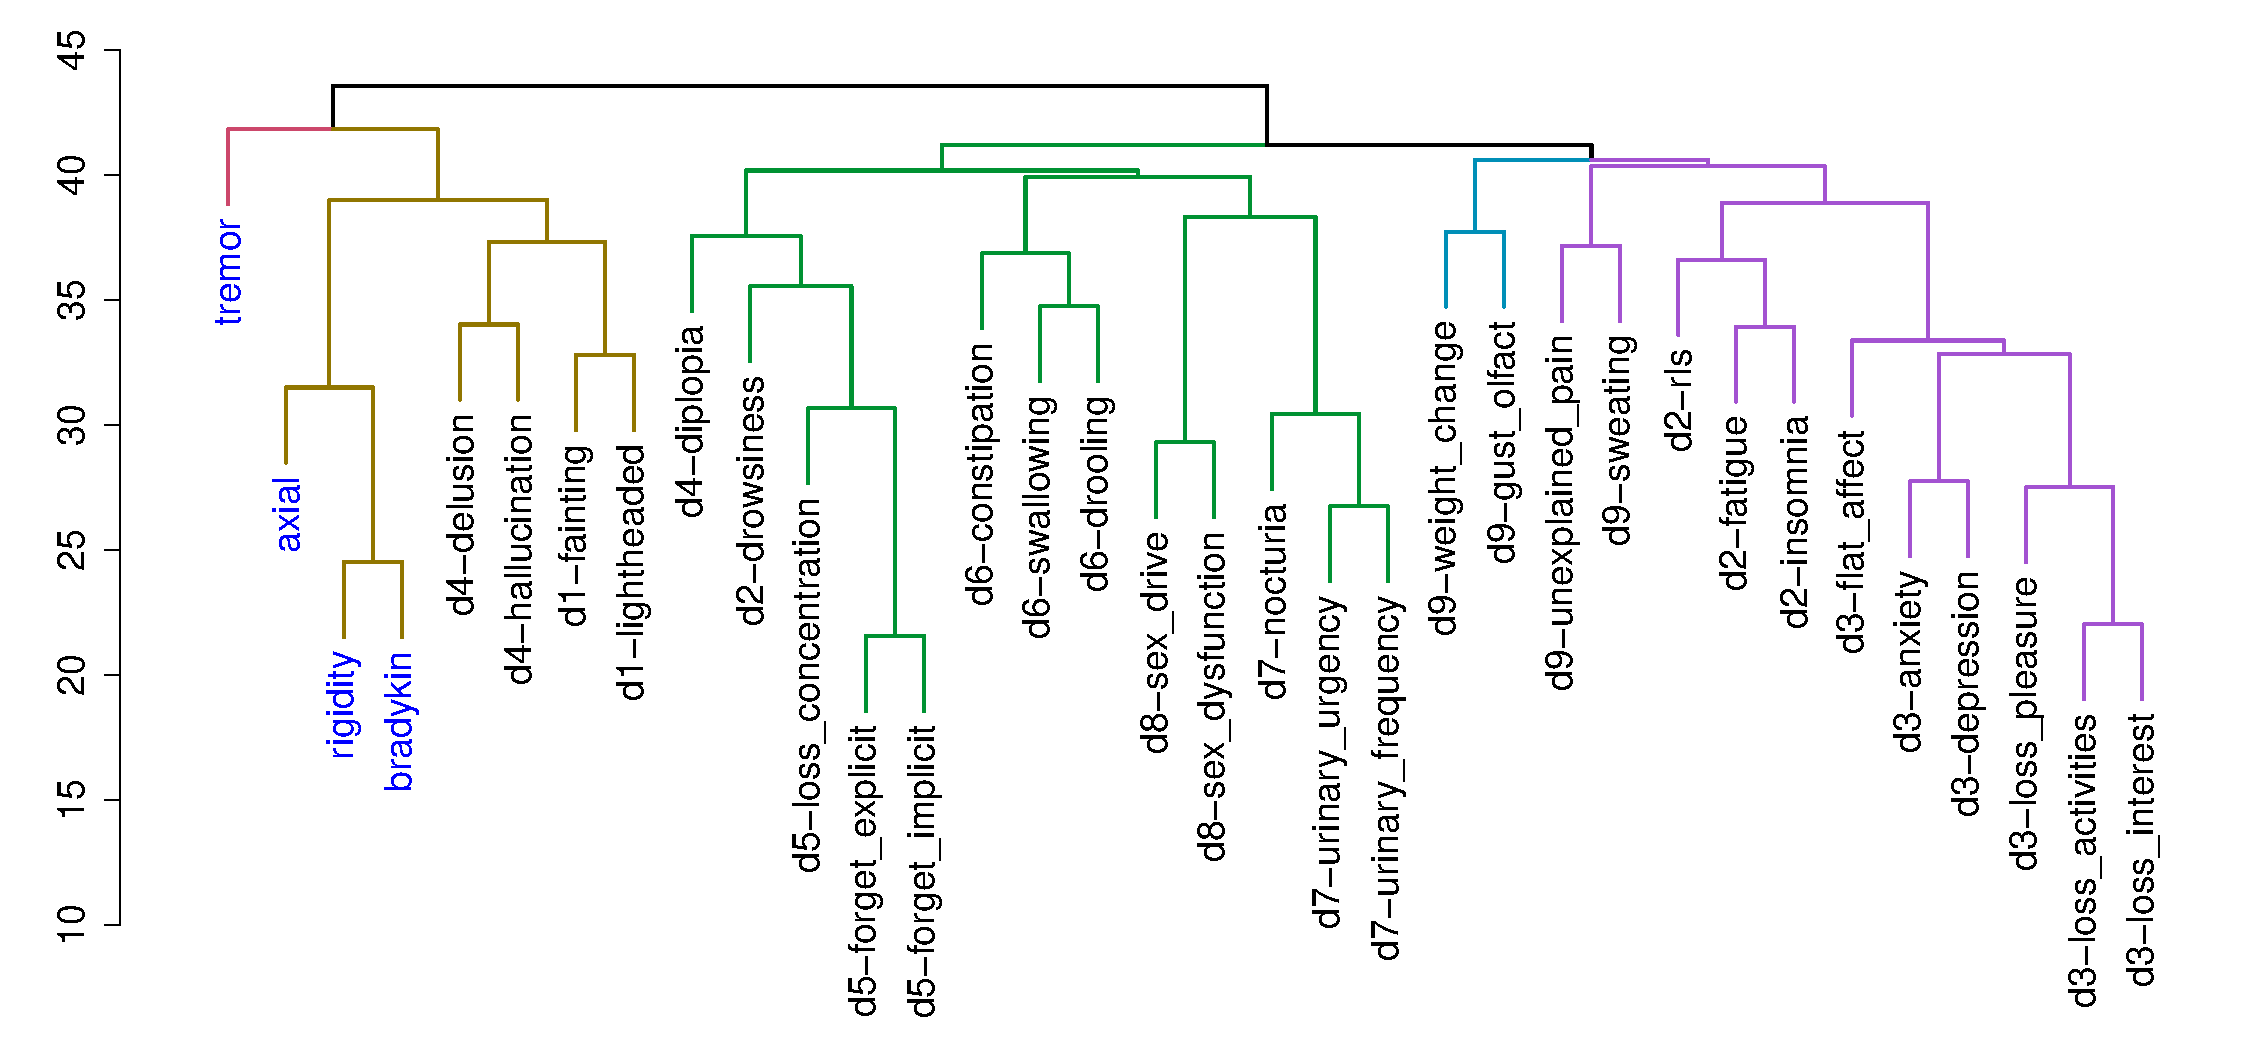
\includegraphics[width=\linewidth]{nms30m-colhc-pub.pdf}
  \caption{Hierarchical clustering of motor (blue) and nonmotor (black) symptoms. Symptoms are
  labeled with their name and corresponding domain number. Dendrogram colored with 5 clusters.}
  \label{fig:hc}
\end{figure*}

% TODO: If the outline of the paper is good enough it might be possible to have this inline
% in the paper somewhere. If so, change figure* -> figure, make h! (force horizontal?), and switch
% 0.8 linewidth to full linewidth
% Also, I'm going to include this AFTER nms30m-colhc, so that colhc/boxplots fits nicely on one
% page
\begin{figure*}[p]
  \centering
  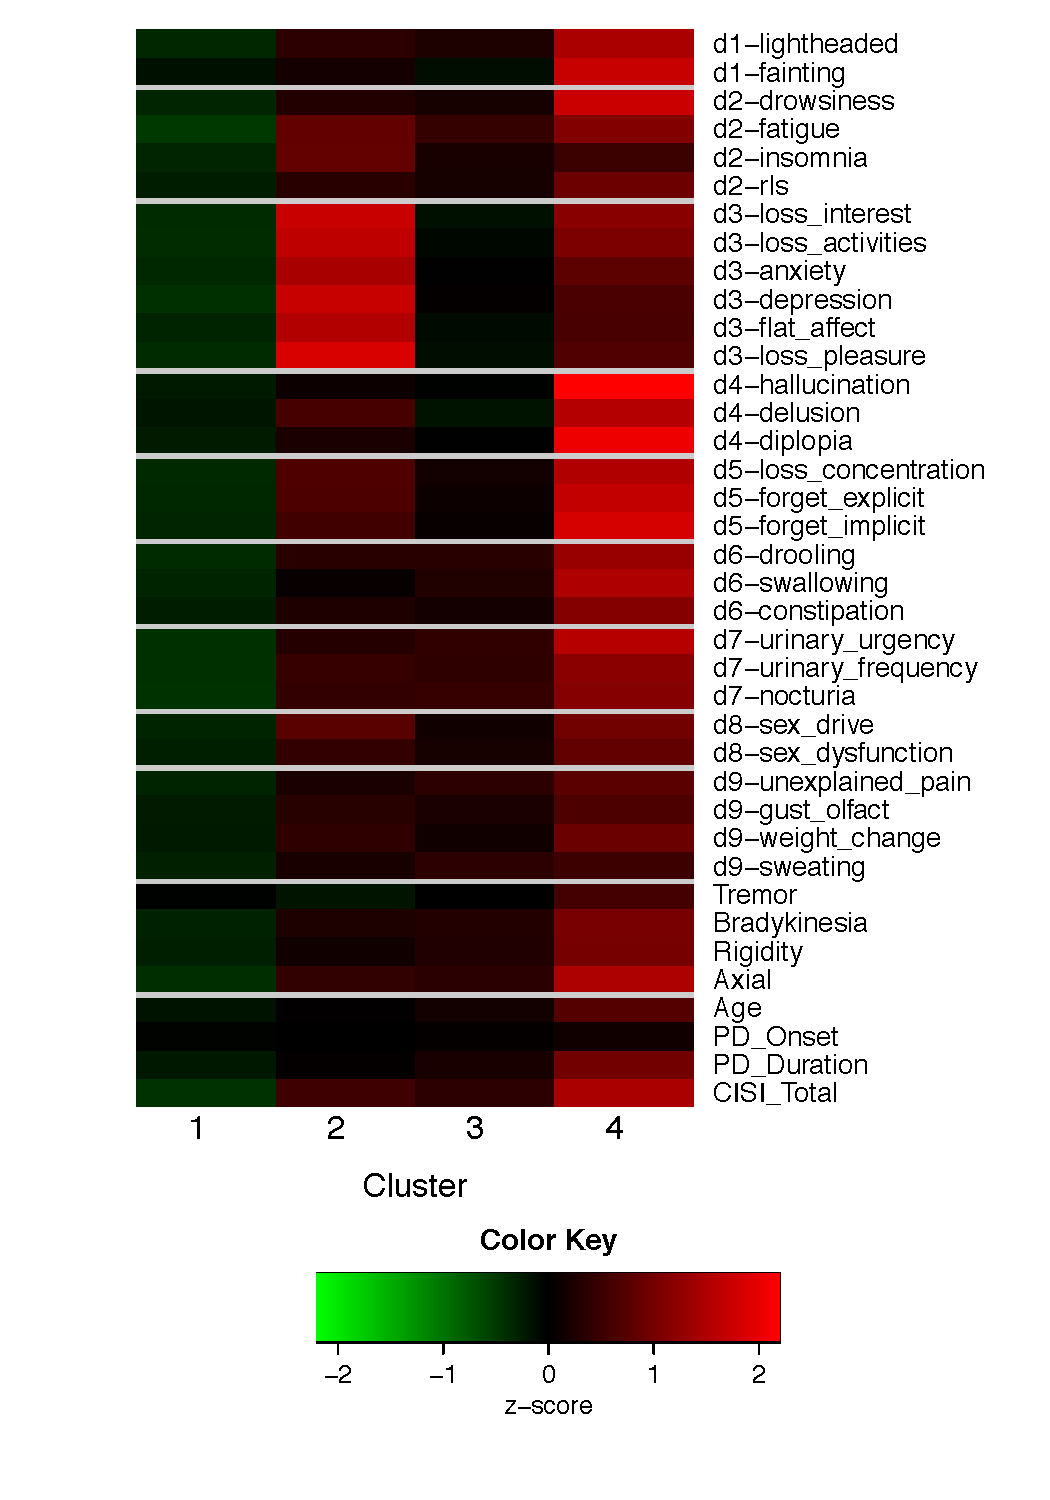
\includegraphics[width=0.7\linewidth]{nms30-hm-pub.pdf}
  % TODO: Variables not used in analysis? Label color - black nms, blue nonmotor, grey ?
  \caption{Heatmap of symptoms clustering. Color indicates cluster mean as a $z$-score for the
  given symptom.}
  \label{fig:nms30-hm}
\end{figure*}

\subsection{Hierarchical clustering on symptoms}

Hierarchical clustering on the 30 nonmotor symptoms and the four motor symptoms produced the
dendrogram in Figure~\ref{fig:hc}. Predictably, symptoms in the same nonmotor domains tended to
cluster together, with the exceptions of diplopia (domain 4) and drowsiness (domain 2), which were
grouped with the attention/memory symptoms of domain 5.  Notably, tremor was the most dissimilar
symptom, occupying a single branch at the top of the tree.

\subsection{Longitudinal analysis}

Most variables had little to no correlation with PD duration (Supplementary Figure~\ref{fig:corr}).
Variables with the highest correlation included symptoms urinary frequency, swallowing, and
drooling; domains miscellaneous, urinary, and gastrointestinal; and total CISI score. Scatterplots
for CISI Total, Tremor, Anxiety, and Depression appear in Supplementary Figure~\ref{fig:long4}.
Total CISI score increased predictably for all four clusters with increasing PD duration, but
tremor, anxiety, and depression had no significant longitudinal progression; indeed, for cluster
2, mood/apathy symptoms appeared to be highest at PD onset, decreasing as time progressed. Notably,
for the motor/nonmotor-dominant groups, differences in severity for motor and nonmotor symptoms
respectively was present early at PD onset, persisting throughout the range of PD durations
observed.

\section{Discussion}

Domains clustering reveals clusters that confirm previous
findings in the field, mainly van Rooden et al.\cite{vanrooden11} and the identification of four
subtypes of Parkinson's disease: mild, nonmotor-dominant, motor-dominant, and severe. van
Rooden's work was conducted with a separate dataset using a different modeling method
(expectation-maximization), and this investigation independently confirms these subtype
classifications. Unlike van Rooden, mean disease durations differences do exist between subtypes 1
(mild) and 4 (severe), likely due to further development of the disease, although the differences
between 2 and 3 (nonmotor/motor predominated) subtypes are insignificant
(Table~\ref{tab:nmd}), importantly suggesting different developmental paths of the disease.

Overall, little information was found in PD onset, PD duration, or current age. Mean ages were
similar for clusters 1, 2, and 3 ($p > 0.05$), but different for the severe cluster 4, intuitively
since cluster 4 represents a more advanced stage of the disease.  Specifically, clusters 1 and 4
seem to be phenotypically quite similar, except at different stages of disease progression, given
cluster 4's higher age and PD duration scores.

However, clusters 2 and 3 clearly show different disease progression, one in
the motor direction, and one in the nonmotor. Both groups have similar age,
PD onset, and PD duration scores, but differ significantly in symptomatic expression.
Cluster 2 is dominated by a high severity of nonmotor domains, especially Sleep/Fatigue,
Mood/apathy, Urinary, and Miscellaneous.  Cluster 3, however, is dominated by a high prevalence
of motor symptoms, where most motor symptoms are similar to the mild cluster 1. Of note is that the
tremor population mean is the highest cluster mean, even higher than the severe subtype 4. This
motor-dominant cluster may thus overlap with Ma et al.'s tremor dominant/slow progression
cluster.\cite{ma15}

Generally, given stable PD onset scores and predictably increasing PD duration
scores for clusters 1 and 4, Ma et al.'s rapid disease
progression/late onset and tremor dominant/slow progression clusters were mostly not found in this
dataset, save for the tremor-dominant motor cluster.

% The most important nonmotor symptoms in determining these clusters were nms\_d2
% (sleep) and nms\_d3 (mood/cognition), which echo findings of Fereshtehnejad's
% longitudinal study\cite{fereshtehnejad15} and are similar to Sauerbier's
% identification of sleep dominant and cognitive dominant clinical NMS subtypes\cite{sauerbier15}.
% Compared to Erro et al.\cite{erro13}, nonmotor/motor
% dominant subtypes were indeed found, but an additional subgroup with relatively
% severe levels of both motor and nonmotor symptoms were found. Erro's benign
% subtype groups possibly overlap with the mild cluster 1 found in this
% investigation.

% \subsection{Nonmotor subtype: clustering and modeling}

% Nonmotor symptoms nms\_d2 and nms\_d3 became critical not only in
% classification trees distinguishing between the various symptoms but in the
% nonmotor-predominant subgroup itself. In $k$-means subdivision of the
% nonmotor-dominant subtype where $k = 2$ and $k = 3$, opposite trends were
% confirmed with nms\_d2 and nms\_d3 symptoms. Similarly, in the 2 and 4 vs rest
% decision tree (Figure~\ref{fig:dtree-2and4va-pruned}), nms\_d2 and nms\_d3 nodes were
% used to differentiate various categories of nomotor-dominant patients.
% When $k = 3$, the subtype with the highest nms\_d2 scores and lowest
% nms\_d3 scores had by far the highest axial scores, nms\_d6 (gastrointestinal)
% scores, and nms\_d7 (urinary) scores. Thus subtype 3 of the nonmotor-dominated
% group could include patients falling into the cognitive/depression-dominant or
% autonomic dominant subtypes.

% Despite the variety in symptomatic expression in this nonmotor group, what
% seems most consistent is the presence of nms\_d9 (miscellaneous) nonmotor
% symptoms, as it is used as the root node of the 2 vs all decision tree
% (Figure~\ref{fig:2va}) and the 2 and 4 vs rest decision tree
% (Figure~\ref{fig:dtree-2and4va-pruned}).

Our longitudinal analysis gives more insight into the clusters found in the previous analyses.
According to Supplementary Figure~\ref{fig:corr}, most symptoms are uncorrelated with PD duration, especially
Mood/apathy symptoms (anxiety, depression) and tremor.
The differences in disease progression for each cluster can be seen by the corresponding graphs in
Figure~\ref{fig:long4}. Cluster 2 (Nonmotor-Dominant) starts at higher
scores for anxiety and depression, and actually decreases with increasing PD duration, thus indicating that these patients' subtype can be determined
early after PD onset from the depressive symptom score. Similarly, when examining cluster 3
(Motor-dominant), the mean tremor score is substantially higher from PD onset.
Interestingly, cluster 4 (Severe) generally starts at lower tremor and motor scores during disease,
but then rises sharply, exceeding other clusters. More evidence that tremor is a unique motor
symptom is located in Figure~\ref{fig:hc}, where it is the most distant symptom from all other
symptoms.

% Indeed, PCA on the 30 nonmotor symptoms identifies the second-most prominent component as a general
% mood/cognition component, and $k$-means clustering on the 30 symptoms only
% (Figure~\ref{fig:nms30m-k4-heatmap-improved}) divides the 1000 patients into four slightly
% different groups, a mild, average, depression-dominant, and severe group.

% The Gaussian mixture model identified in Figure~\ref{fig:nms30m-mclust-heatmap-improved} fragments
% the previously-discovered clusters into more groups. Here, a wide variety of specialized subtypes
% of PD are displayed, including insomnia, urinary, motor, nonmotor, and depression-dominant groups,
% as well as the expected mild, average, and severe subtypes. It is likely that the previous analysis
% with only nms\_d\{1-9\} combined most of those specialized groups into the more general
% nonmotor-dominant Subtype 2.

It's intuitive that a Depression-Dominant group emerges from the symptoms clustering, since the
Mood/apathy domain consists of 5 separate measures. Thus, any high expression of depressive
symptoms is magnified in clustering, since the symptoms are highly similar (Figure~\ref{fig:hc})
and treated with equal weight. Once again reinforcing what was discovered previously, depressive
symptoms have been shown to be very important in determining subtypes of PD.

\section{Supplementary Material}

\begin{suppfigure}[h]
  \centering
  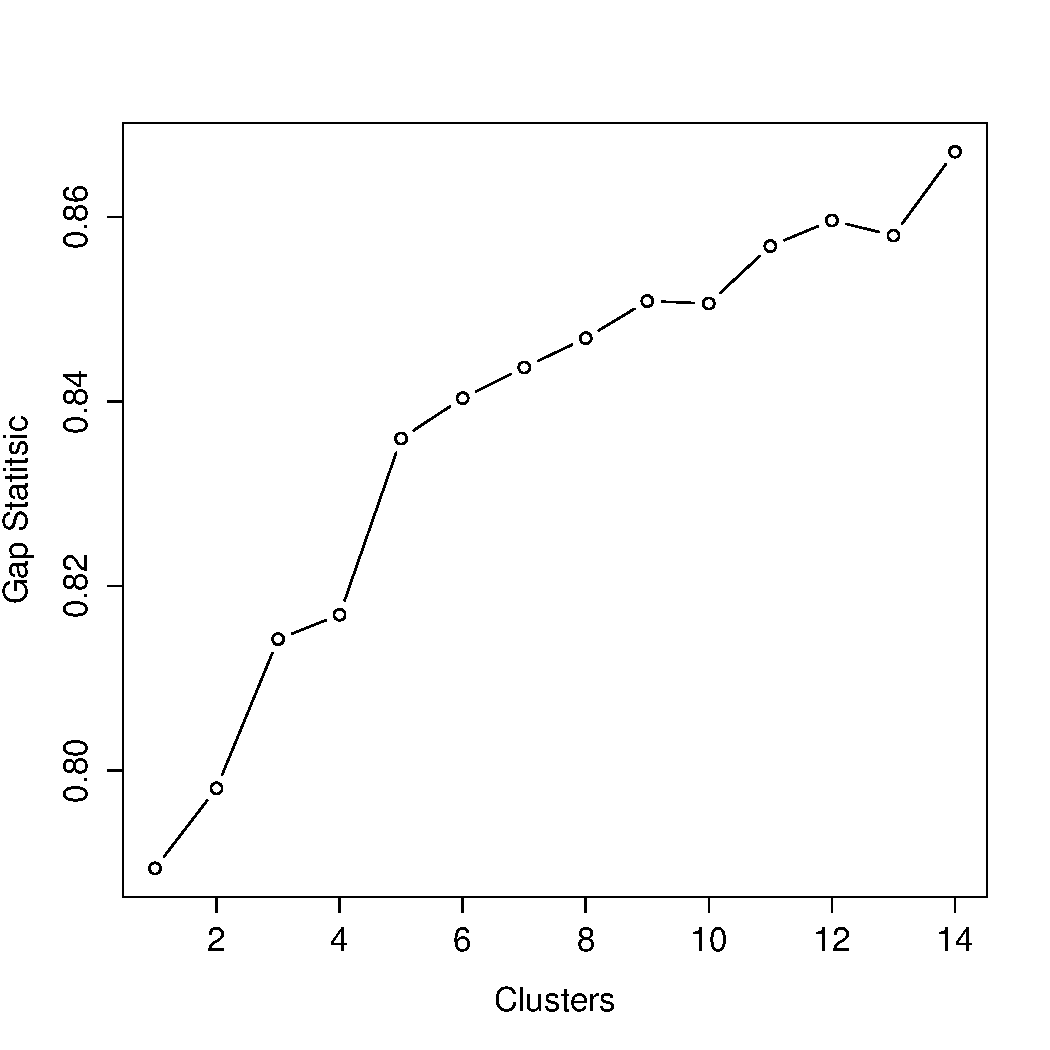
\includegraphics[width=\linewidth]{gap-statistic.pdf}
  \caption{Plot of the gap statistic $\text{Gap}(k)$ versus number of clusters with $k$-means on
  500 bootstrapped samples of the domains clustering. Error bars represent $\pm$ 1 standard error
  (se). Per the method described in Tibshirani,\cite{tibshirani01gap} the optimal number of
  clusters is the smallest $k$ such that $\text{Gap}(k) \geq \text{Gap}(k + 1) - \text{se}_{k +
  1}$. In this case, $k = 4$.}
  \label{fig:gap}
\end{suppfigure}

\begin{suppfigure*}[p]
  \centering
  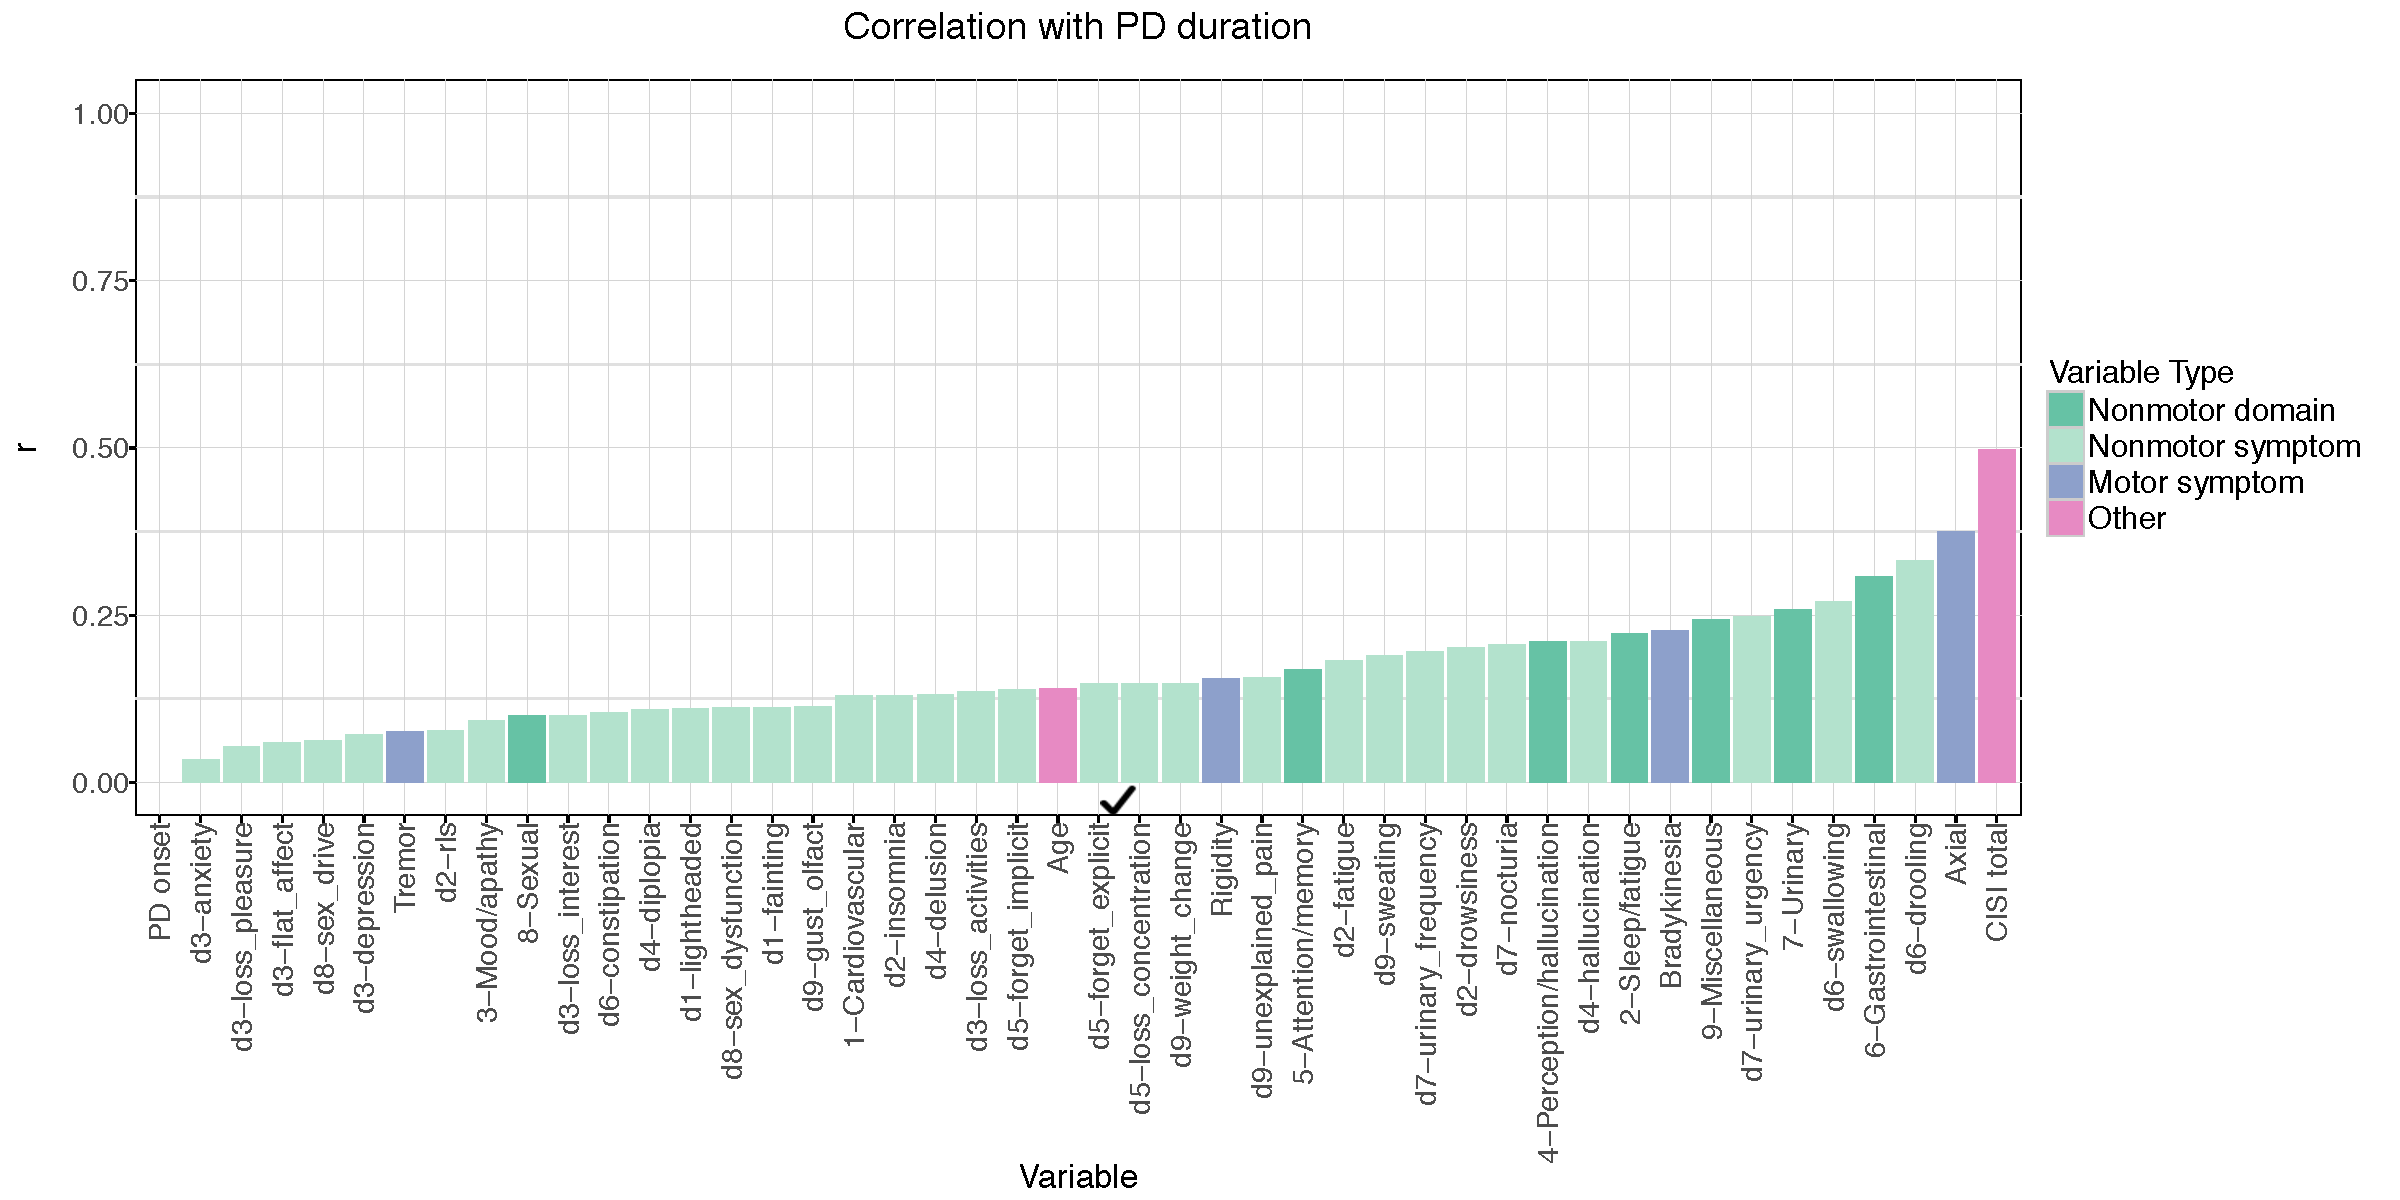
\includegraphics[width=\linewidth]{cor-unbinned.pdf}
  \caption{Correlation of each symptom with PD duration.}
  \label{fig:corr}
\end{suppfigure*}

\begin{suppfigure*}[p]
  \centering
  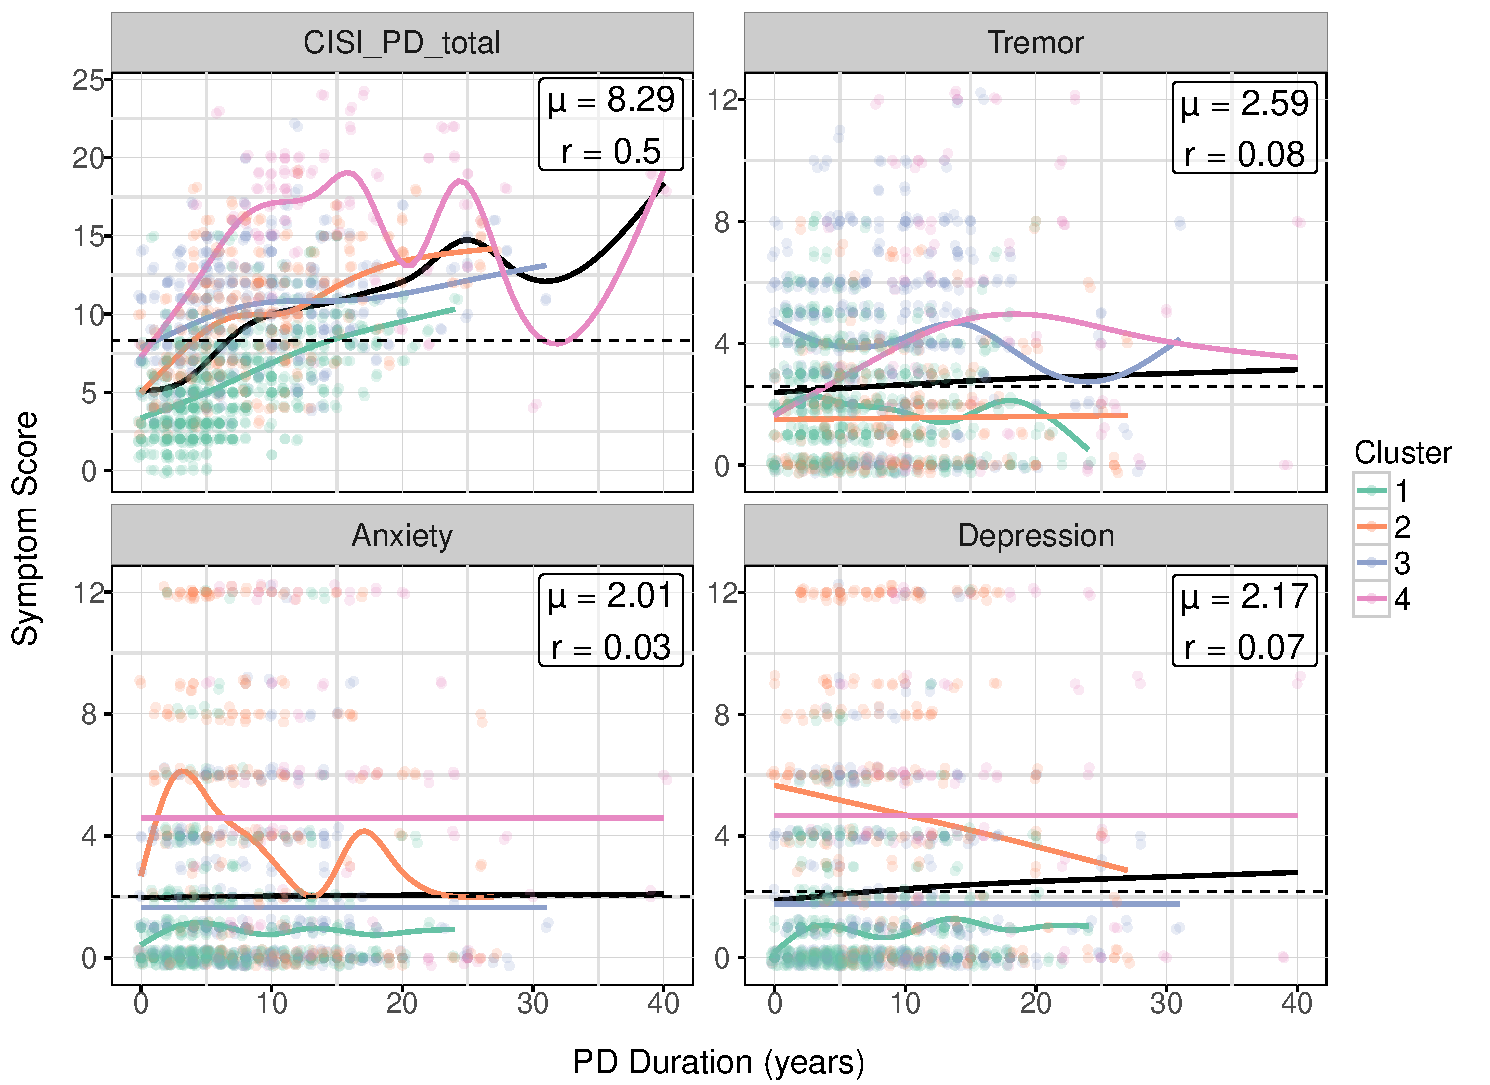
\includegraphics[width=0.8\linewidth]{long4-d.pdf}
  % TODO: Get rid of capital T in  CISI Total
  \caption{Selected symptoms plotted against PD duration. Smoothed loess curves for each cluster
  are drawn in their respective colors. The black curve is the curve for the entire population, and
the global mean score is marked with a dotted line.}
  \label{fig:long4}
\end{suppfigure*}


\section{References}

\bibliography{manuscript}

\end{document}
